
http://rstudio-pubs-static.s3.amazonaws.com/8753_a57d3950027541a590c9b40a045accbf.html#15

\begin{frame}{Why learn to use a SQLite database?}

	\begin{itemize}
		\item You already know SQL.
		\item A normalized database structure is appropriate for the data.
		\item You want to reduce memory requirements.
		\item You are using an R package or script that is database-aware.
		\item You want to share data with another application like PHP.
	\end{itemize}
\end{frame}



\begin{frame}{What is different about SQLite?
}

	\begin{itemize}
		\item SQLite can be called from other software (like R) without requiring any installation.
		\item SQLite does not require server administration.
		\item Data is stored in a single, cross-platform file.
		\item SQLite is in the public domain.
		\item Database sizes up to 140Tb are possible.
	 \item SQLite is considered the most widely used database.
	\end{itemize}
\end{frame}



\begin{frame}{Packages required for database interaction}
\begin{itemize}
		\item sqldf - Like using SQL queries? Use SQL syntax with R dataframes.
	\item  DBI - Basic functions to connect to all types of external databases
	\item  RSQLite - Functions to embed SQLite into R
	\item  RSQLite.extfuns - Include some SQLite extensions
	\end{itemize}
\end{frame}



\begin{frame}{Basic database and table creation}

library(DBI)
library(RSQLite)
# This connection creates an empty database if it does not exist
db <- dbConnect(SQLite(), dbname = "./Test.sqlite")
dbSendQuery(conn = db, "CREATE TABLE School(SchID INTERGER, Location Text,
Authority TEXT, SchSize TEXT)")

## <SQLiteResult: DBI RES (843, 0, 1)>

\end{frame}


Basic database and table creation

library(DBI)
library(RSQLite)
# This connection creates an empty database if it does not exist
db <- dbConnect(SQLite(), dbname = "./Test.sqlite")
dbSendQuery(conn = db, "CREATE TABLE School(SchID INTERGER, Location Text,
Authority TEXT, SchSize TEXT)")

## <SQLiteResult: DBI RES (843, 0, 1)>

\begin{frame}{Populate table with SQL commands}

dbSendQuery(conn = db, "INSERT INTO School values (1,'urban', 'state', 'medium')")


## <SQLiteResult: DBI RES (843, 0, 2)>


dbSendQuery(conn = db, "INSERT INTO School values (2,'urban', 'independent', 'large')")


## <SQLiteResult: DBI RES (843, 0, 3)>
\end{frame}



\begin{frame}{Populate table from a dataframe objec}
If your data already resides in an R dataframe...


# Load your R dataframe
load(file = "~/RProject/sqlite/DATA/Class.rda")
# Push to SQLite
dbWriteTable(conn = db, name = "Class", value = Class, row.names = FALSE)

## [1] TRUE


\end{frame}



Populate table from csv file

dbWriteTable(conn = db, name = "Student", value = "~/RProject/sqlite/DATA/student.csv",
    row.names = FALSE, header = TRUE)

## [1] TRUE


dbListFields(db, "Student")

## [1] "studID"  "classID" "Gender"  "Test1"   "Test2"

Check out the functions from the XLConnect package that could read this data into SQLite from a 3 worksheet Excel file.


\begin{center}
	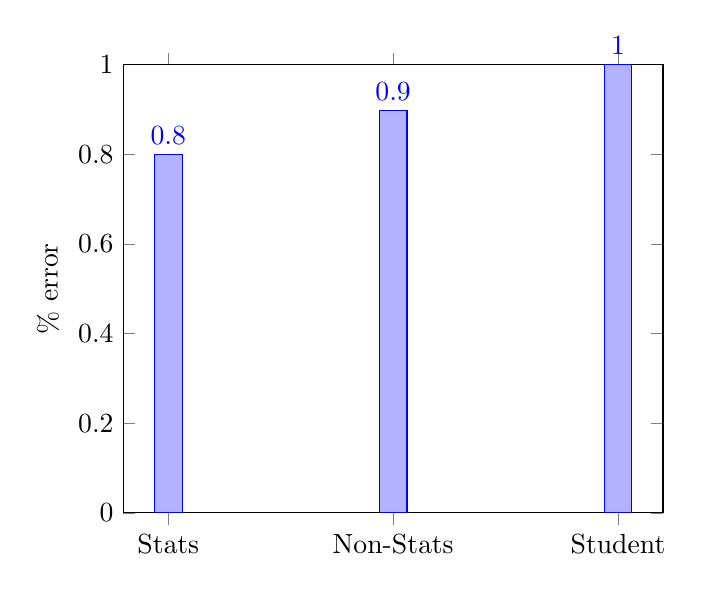
\begin{tikzpicture}
		\begin{axis}[
			ymin=0, ymax = 1,
    			ybar,
    			ylabel={\% error},
    			symbolic x coords={Stats,Non-Stats,Student},
    			xtick=data,
    			nodes near coords,
    			nodes near coords align={vertical},
    			]
			\addplot coordinates {(Stats,.8) (Non-Stats,.897) (Student,1)};
		\end{axis}
	\end{tikzpicture}
\end{center}
\end{frame}
\begin{frame}
Similar:
	\begin{description}
		\item[Oakes (1986)] 97\% Error rate
		\item[Falk and Greenbaum (1995)] 87\% Error rate
	\end{description}
\end{frame}

% The p-value
\begin{frame}{Hypothesis Testing}
	\begin{itemize}
		\pause
		\item Let $X$ be a random sample of size $n$ from a distribution with
			  finite mean $\mu$ and variance $\sigma^2$. Then (by central limit theorem)
			 \[\bar{X} \xrightarrow{d} \mathrm{N}\left (\mu, \frac{\sigma^2}{n}\right )\]
		\pause
		\item So, if the true mean $\mu$ is zero, then $\bar{X}$ is (approximately)
			  normally distributed with mean $0$ and standard deviation
			  $\frac{\sigma}{\sqrt{n}}$.
		\pause
		\item If this is unlikely, then "reject the null".
	\end{itemize}
\end{frame}

\begin{frame}{The p-value is uninteresting}
Setup:
	\begin{itemize}
		\item Police force in a city of 1,000,000 people with 100 criminals
		\item Lie detector with 99\% accuracy
		\item $H_0$: Person is innocent
	\end{itemize}
Experiment:
	\begin{itemize}
		\item Test one person and find guilty.
		\item p-value?
		\pause
		\begin{itemize}
			\item 1\% false positive rate, so $p = 0.01$.
		\end{itemize}
		\pause
		\item Probability that person is actually guilty?
		\pause
		\begin{align*}
			P(H_1|D) &= \frac{P(D|H_1)P(H_1)}{P(D)} \\
					 &= \frac{0.99 \cdot 0.0001}
					   		 {0.99 \cdot 0.0001 + 0.01 \cdot 0.9999} \\
					 &\approx 0.001
		\end{align*}
	\end{itemize}
\end{frame}

\begin{frame}{The Case for Bayes}
	\begin{itemize}
		\item Gives us what we want: The probability that a hypothesis is true.
		\item Allows us to specify more complex/realistic models.
		\item Allows us to incorporate prior information/research.
	\end{itemize}
\end{frame}
